\section{Experimental Evaluation}
\label{sec:experiments}
In this section we present both qualitative and quantitative  performance evaluations of visual MPC on various manipulation tasks assessing the degree of generalization and comparing different prediction models and cost functions and with a hand-crafted baseline.
In Figures \ref{fig:example_traj} and \ref{fig:tile_2} we present a set of qualitative experiments showing that visual MPC trained fully self-supervised is capable of solving a wide range of complex tasks.
Videos for the qualitative examples are at the following webpage\footnote{For videos, see \url{https://sites.google.com/view/visualforesight/}}.
In order to perform quantitative comparisons, we define a set of tasks where the robot is required to move object(s) into a goal configuration. For measuring success, we use a distance-based evaluation where a human annotates the positions of the objects after pushing allowing us to compute the remaining distance to the goal.

\subsection{Comparing Video Prediction Architectures}
\label{subsec:sna_experiments}
We first aim to answer the question: Does  visual MPC using the occlusion-aware SNA video prediction model that includes temporal skip connections outperform visual MPC with the dynamic neural advection model (DNA)\cite{foresight} \emph{without} temporal skip-connections?

\begin{table}
\centering
{\footnotesize
\begin{tabular}{lcc}
	\toprule
         &  \thead{moved imp. \\ $\pm$ std err. of mean} &   \thead{stationary imp. \\ $\pm$ std err. of mean}  \\
         \midrule
  DNA \cite{foresight} & 0.83 $\pm$0.25 &  -1.1 $\pm$ 0.2\\ 
  SNA & \textbf{10.6 $\pm$ 0.82} & \textbf{-1.5 $\pm$ 0.2} \\
  \bottomrule
\end{tabular}
}
\caption{Results for multi-objective pushing on 8 object/goal configurations with 2 seen and 2 novel objects. Values indicate improvement in distance from starting position, higher is better. Units are pixels in the 64x64 images.} 
\label{table:mult_obj}
\end{table}
To examine whether our skip-connection model (SNA) helps with handling occlusions, we devised a task that requires the robot to push one object, while keeping another object stationary. When the stationary object is in the way, the robot must move the target object around it. This is illustrated on the left side of \autoref{fig:goingaroundocclusion} in the appendix. While pushing the target object, the gripper may occlude the stationary object, and the task can only be performed successfully if the model can make accurate predictions through this occlusion. These tasks are specified by selecting one starting pixel on the target object, a goal pixel location for the target object, and commanding the obstacle to remain stationary by selecting the same pixel on the obstacle for both start and goal. 

We use four different object arrangements with two training objects and two objects that were not seen during training. We find that, in most cases, the SNA model is able to find a valid trajectory, while the DNA model, that is not able to handle occlusion, is mostly unable to find a solution. The results of our quantitative comparisons are shown in \autoref{table:mult_obj}, indicating that temporal skip-connections indeed help with handling occlusion in combined pushing and obstacle avoidance tasks. 

\subsection{Evaluating Registration-Based Cost Functions}
\label{susbsec:reg_cost_exp}

\begin{table}
	{\footnotesize
		\begin{center}
			\begin{tabular}{lcc}
				\toprule
				%				 & \multicolumn{2}{c}{fraction of successful runs} \\
				& Short & Long \\
				\midrule
				Visual MPC $+$ predictor propagation  & 83\% & 20\% \\
				Visual MPC $+$ OpenCV tracking  & 83\%  & 45\% \\
				Visual MPC $+$ registration network & 83\% & \textbf{66\%}  \\
				\bottomrule
			\end{tabular}
		\end{center}
	}
	\caption{\small Success rate for long-distance pushing experiment with 20 different object/goal configurations and short-distance experiment with 15 object/goal configurations. Success is defined as bringing the object closer than 15 pixels to the goal, which corresponds to around $7.5cm$.}
	\label{table:res_long_short}
\end{table}
In this section we ask: How important  is it to update the model's belief of where the target objects currently are? 
We first provide two qualitative examples: In example (5)-(6) of Figure \ref{fig:tile_2} the task is to bring the stuffed animal to a particular location in 3D-space on the other side of the arena. To test the system's reaction to perturbations that could be encountered in open-world settings, during execution a person knocks the object out of the robot's hand (in the 3rd frame). The experiment shows that visual MPC is able to naturally perform a new grasp attempt and bring the object to the goal. This trajectory is easier to view in the supplementary video.

In Figure \ref{fig:push_retry} in the appendix, the task is to push the bottle to the point marked with the green dot. In the beginning of the trajectory the object behaves differently than expected, it moves downwards instead of to the right. However the system recovers from the initial failure and still pushes the object to the goal.

The next question we investigate is: How much does tracking the target object using the learned registration matter for short horizon versus long horizon tasks? 
In this experiment, we disable the gripper control, which requires the robot to push objects to the target. We compare two variants of updating the positions of the designated pixel when using a pixel-distance based cost function. The first is a cost function that uses our registration-based method, trained in a fully self-supervised fashion, and the second is with a cost function that uses off-the shelf tracking from OpenCV \cite{babenko2009visual}. Additionally we compare to visual MPC,
%%SL.11.21: isn't it all visual MPC?
which uses the video-prediction model's own prior predictions to update the current position of the designated pixel, rather than tracking the object with registration or tracking.

We evaluate our method on 20 long-distance and 15 short-distance pushing tasks. For long distance tasks the initial distance between the object and its goal position is $30cm$ while for short distance tasks it is $15cm$. Table \ref{table:res_long_short} lists quantitative comparisons showing that on the long distance experiment
visual MPC using the registration-based cost not only outperforms prior work \cite{sna}, but also outperforms the hand-designed, supervised object tracker \cite{babenko2009visual}. By contrast, for the short distance experiment,
all methods perform comparably. Thus, theses results demonstrate the importance of tracking the position of the target object for \emph{long-horizon tasks}, while for short-horizon tasks object tracking appears to be irrelevant. 
\subsection{Evaluating Classifier-Based Cost Function}
\label{subsec:eval_classifier}

\begin{figure}
	\centering
	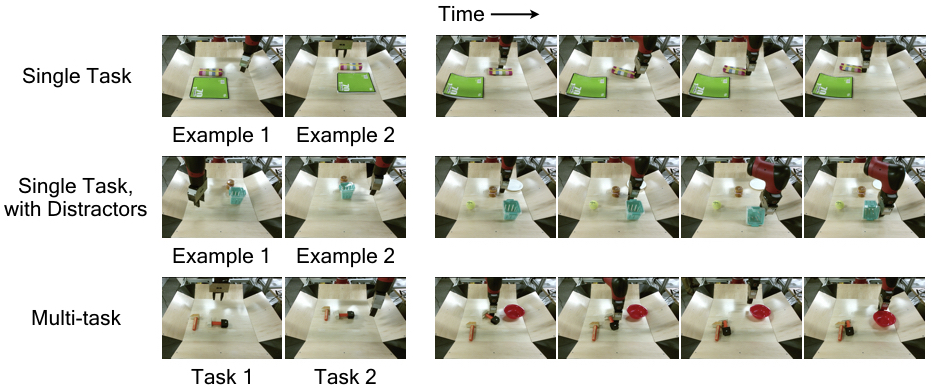
\includegraphics[width=1.0\columnwidth]{images_cls/cls_results_3.jpeg}
	\caption{\small Object arrangement performance of our goal classifier with distractor objects and with two tasks. The left shows a subset of the 5 positive examples that are provided for inferring the goal classifier(s), while the right shows the robot executing the specified task(s) via visual planning.}
	\label{fig:cls_results}
	\vspace{-0.3cm}
\end{figure}

The goal of the classifier-based cost function is to provide an easy way to compute an objective for new tasks from a few observations of success for that task, so we compare our approach to alternative and prior methods for doing so under the same assumptions: pixel distance and latent space distance. In the latter, we measure the distance between the current and goal observations in a learned latent space, obtained by training an autoencoder (DSAE) \cite{dsae} on the same data used for our classifier. Since we are considering a different form of task specification incompatible with user-specified pixels, we do not compare the classifier-based cost function to the cost function based on designated pixels.

To collect data for meta-training the classifier, we randomly select a pair of objects from our set of training objects, and position them in many different relative positions, recording the image for each configuration. Each task corresponds to a particular relative positioning of two objects, e.g. the first object to the left of the second, and we construct positive and negative examples for each task by labeling the aforementioned images. We randomly position the arm in each image, as it is not a determiner of task success. A good classifier should ignore the position of the arm. We also include randomly-positioned distractor objects in about a third of the collected images.

We evaluate the classifier-based cost function in three different experimental settings. In the first setting, the goal is to arrange two objects into a specified relative arrangement. The second setting is the same, but with distractor objects present. In the final and most challenging setting, the goal is to achieve two tasks in sequence. We provide positive examples for both tasks, infer the classifier for both, perform MPC for the first task until completion, followed by MPC for the second task. The arrangements of the evaluation tasks were chosen among the eight principal directions (N, NE, E, SE, etc.). To evaluate the ability to generalize to new goals and settings, we use novel, held-out objects for all of the task and distractor objects in our evaluation.

We qualitatively visualize the tasks in Figure~\ref{fig:cls_results}. On the left, we show a subset of the five images provided to illustrate the task(s), and on the left, we show the motions performed by the robot. We see that the robot is able to execute motions which lead to a correct relative positioning of the objects.
We quantitatively evaluate the three cost functions across 20 tasks, including $10$ unique object pairs. A task was considered successfully completed if more than half of the object was correctly positioned relative to the other. The results, shown in Figure~\ref{fig:cls_charts}, indicate that the distance-based metrics struggle to infer the goal of the task, while our approach leads to substantially more successful behavior on average.

\begin{figure}
    \centering
    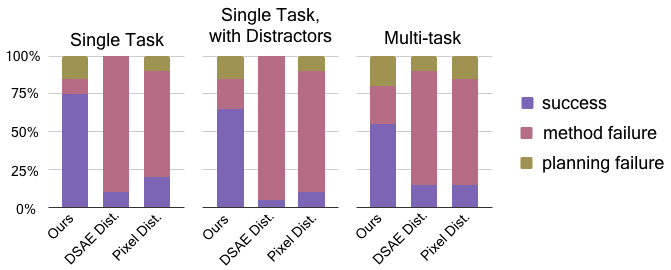
\includegraphics[width=0.48\textwidth]{images_cls/cls_charts_2.jpeg}
    \caption{\small Quantitative performance of visual planning for object rearrangement tasks across different goal specification methods: our meta-learned classifier, DSAE~\cite{dsae}, and pixel error. Where possible, we include break down the cause of failures into errors caused by inaccurate prediction or planning and those caused by an inaccurate goal classifier.}
    \label{fig:cls_charts}
    \vspace{-0.3cm}
\end{figure}


\subsection{Evaluating Multi-Task Performance}
\label{subsec:multi_task_bench}
One of the key motivations for visual MPC is to build a system that can solve a \emph{wide variety} of different tasks, involving completely different objects, physics and, objectives.
Examples for tasks that can be solved with visual MPC are shown in Figure \ref{fig:example_traj} and \ref{fig:tile_2}. Task 1 in Figure~\ref{fig:example_traj} shows a ``placing task" where an object needs to be grasped and placed onto a plate while not displacing the plate. Task 2 is an object rearrangement tasks. The example shown in Task 4 and all examples in Figure \ref{fig:cls_results} show relative object rearrangement tasks. Examples 5 and 6 show the same 3D object positioning tasks from different views. In Task 7, the goal is to move the black object to the goal location while avoiding the obstacle in the middle which is marked with a designated- and goal pixel. We also demonstrate that visual MPC -- without modifications to the algorithm -- solves tasks involving deformable objects such as a task where a towel needs to be wrapped around an object (Task 3), or folding a pair of shorts (Task 8). To the best of our knowledge this is the first algorithm for robotic manipulation handling both rigid and deformable objects.
For a full illustration of each of these tasks, we encourage the reader to watch the supplementary video.

The generality of visual MPC mainly stems from two components --- the generality of the visual dynamics model and the generality of the task definition.
We found that the dynamics model often generalizes well to objects outside of the training set, if they have similar properties to the objects it was trained with. For example, Task 8 in Figure \ref{fig:tile_2} shows the model predicting a pair of shorts being folded. We observed that a model, which was only provided videos of towels during training, generalized to shorts, although it had never seen them before. In all of the qualitative examples, the predictions are performed by the \emph{same model}.
We found that the model sometimes exhibits confusion about whether an object follows the dynamics of a cloth or rigid objects, which is likely caused by a lack of training data in the particular regime. To overcome this issue we add a binary token to the state vector indicating whether the object in the bin is hard or soft. 
We expect that adding more training data would remove the need for this indicator and allow the model to infer material properties directly from images.

\begin{figure*}
	\centering
	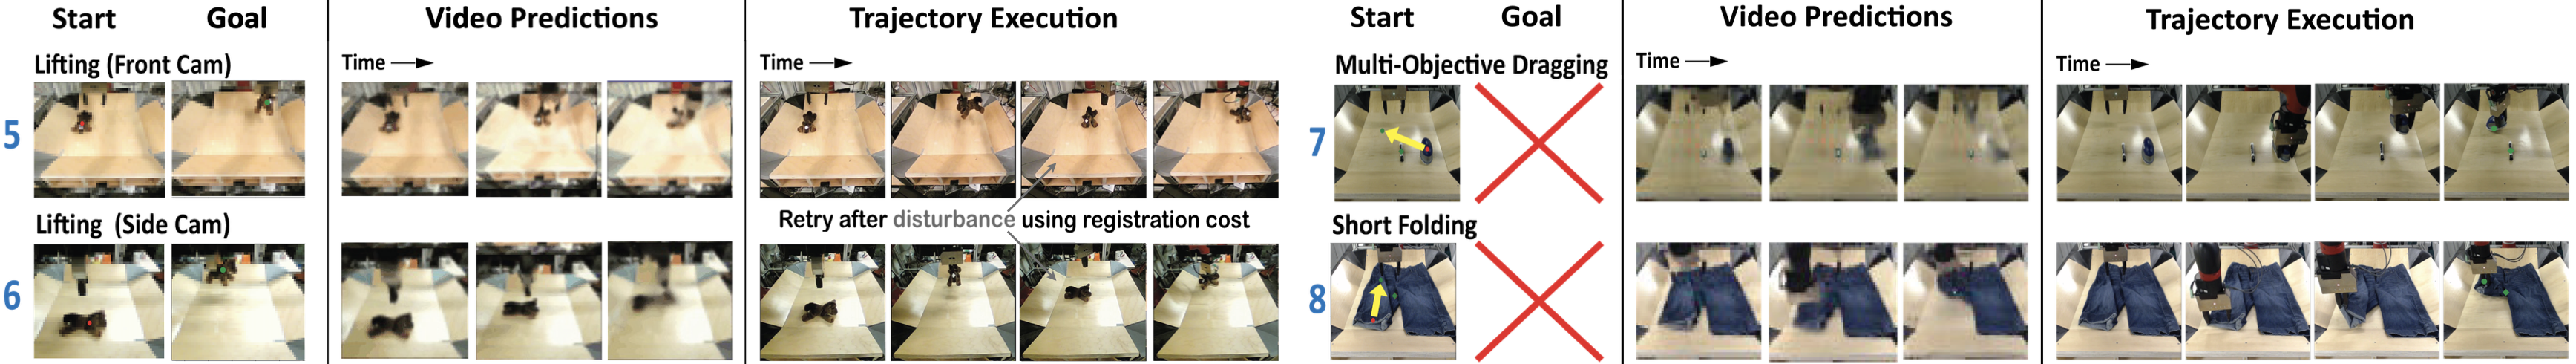
\includegraphics[width=2.05\columnwidth]{images_general/2colfig.png}
	\caption{Visual MPC successfully solves a wide variety of tasks including multi-objective tasks, such as placing an object on a plate (row 5 and 6), object positioning with obstacle avoidance (row 7) and folding shorts (row 8). Zoom in on PDF.   
		\label{fig:tile_2}}
\end{figure*}
% was: {images_general/tile_2.png}

The ability to specify tasks in multiple different ways adds to the flexibility of the proposed system. Using designated pixels, object positioning tasks can be defined in 3D space, as shown in Task 1 and 2 in Figure~\ref{fig:example_traj} and task 5-6 in Figure~\ref{fig:tile_2}. When adding a goal image, the positioning accuracy can be improved by utilizing the registration scheme discussed in Section \ref{subsec:reg_cost}.
For tasks where we care about \emph{relative} rather than absolute positioning, a meta-learned classifier can be used, as discussed in Section \ref{subsec:class_cost}.

Next, we present a quantitative evaluation to answer the following question: How does visual MPC compare to a hand-engineered baseline on a large number of diverse tasks? For this comparison, we engineered a simple trajectory generator to perform a grasp at the location of the initial designated pixel, lift the arm, and bring it to the position of the goal pixel. Camera calibration was performed to carry out the necessary conversions between image-space and robot work-space coordinates, which was not required for our visual MPC method. For simplicity, the baseline controller executes in open loop. Therefore, to allow for a fair comparison, visual MPC is also executed open-loop, i.e. no registration or tracking is used.
Altogether we selected 16 tasks, including the qualitative examples presented earlier.
The quantitative comparison is shown in Table \ref{table:cloth_folding}, illustrating that visual MPC substantially outperforms this baseline.
Visual MPC succeeded for most of the tasks. While the baseline succeeded for some of the cloth folding tasks, it failed for almost all of the object relocation tasks. This indicates that an implicit understanding of physics, as captured by our video prediction models, is indeed essential for performing this diverse range of object relocation and manipulation tasks, and the model must perform non-trivial physical reasoning beyond simply placing and moving the end-effector.




\label{subsec:cloth_folding_data}
\begin{table}
\centering
{\footnotesize
\begin{tabular}{lcc}
	\toprule
         &  \thead{\% of Trials with \\ Final Pixel Distance $< 15$}   \\
         \midrule
  Visual MPC & \textbf{75\%} \\ 
  Calibrated Camera Baseline & 18.75 \% \\
  \bottomrule
\end{tabular}
}
\caption{Results for a multi-task experiment of 10 hard object pushing and grasping tasks, along with 6 cloth folding tasks, evaluating using a single model. Values indicate the percentage of trials that ended with the object pixel closer than 15 pixels to the designated goal. Higher is better.} 
\label{table:cloth_folding}
\end{table}

\subsection{Discussion of Experimental Results}

Generalization to many distinct tasks in visually diverse settings is arguably one of the biggest challenges in reinforcement learning and robotics today. While deep learning has relieved us from much of the problem-specific engineering, most of the works either require extensive amounts of labeled data or focus on the mastery of single tasks while relying on human-provided reward signals. 
From the experiments with visual MPC, especially the qualitative examples and the multi-task experiment, we can conclude that visual MPC \emph{generalizes} to a wide range of tasks it has never seen during training. This is in contrast to many model-free approaches for robotic control which often struggle to perform well on novel tasks. Most of the generalization performance is likely a result of large-scale self-supervised learning, which allows to acquire a rich, task-agnostic dynamics model of the environment. 